\chapter{Lösungsansatz zur Klassifikation}
In diesem Kapitel geht es um die Strategie, wie eine Klassifikation der
Hunderassen für den großen (120 Klassen) und den kleinen (5 Klassen) Datensatz
mittels mehrerer Neuronaler Netze erreicht werden kann.

\section{Größe der Bilder}
Höhe und Breite der Bilder sind unterschiedlich im großen Datensatz, wie in
\autoref{fig:scatter_groß} dargestellt.

\begin{figure}
  \centering
  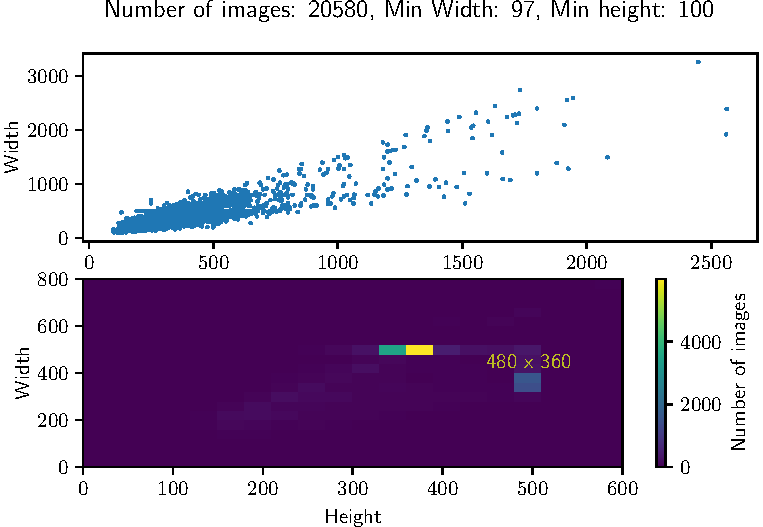
\includegraphics[scale=0.9]{pics/width_height_scatter_hist2d.pdf}
  \caption{Oben: Scatter-Plot der Höhen- und Breitenverteilung der Bilder aus dem großen Datensatz.
  Unten: Zweidimensionales Histogramm der Höhen- und Breitenverteilung.
  Die gelbe Größe entspricht der am häufigsten auftretenden Kombination
  aus Breite und Höhe.}
  \label{fig:scatter_groß}
\end{figure}

Die minimale Breite liegt bei 97 Pixeln und die minimale Höhe bei 100 Pixeln.
Prinzipiell arbeiten die verwendeten Neuronalen Netze ohne definierte Input
size, allerdings müssen die Bilder auf eine Größe gebracht werden, da
\texttt{numpy arrays} eine definierte Größe haben müssen. Eine Möglichkeit wäre
es nun, alle Bilder auf diese minimale Größe zu resizen. Damit würde allerdings
ein Informationsverlust einhergehen. Aus diesem Grund wurde ein zu Teilen
selbstgeschriebener \texttt{Datagenerator} verwendet, der die Bilder batchwise
lädt und batchwise auf das Minimum im Batch resized. Auf diese Weise ist der
Informationsverlust geringer als alle Bilder auf 97x100 zu resizen.

In \autoref{fig:scatter_klein} ist die Höhen- und Breitenverteilung auch für
den kleinen Datensatz dargestellt.

\begin{figure}
  \centering
  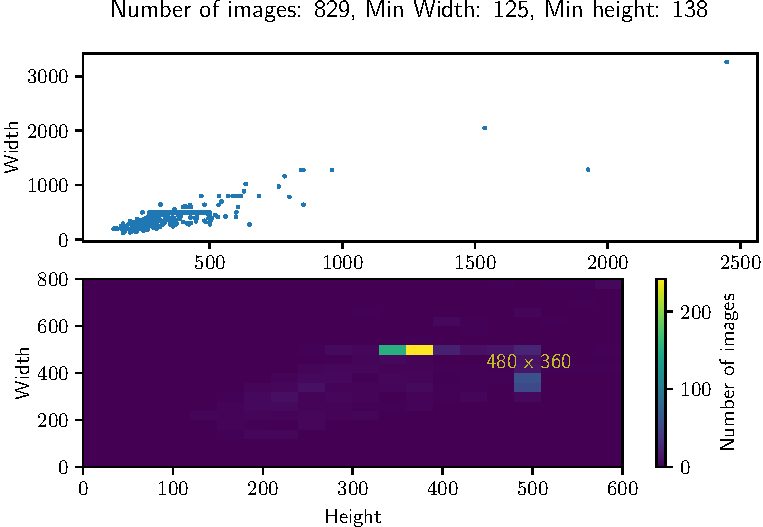
\includegraphics[scale=0.9]{pics/width_height_scatter_hist2d_klein.pdf}
  \caption{Oben: Scatter-Plot der Höhen- und Breitenverteilung der Bilder aus
  dem kleinen Datensatz.
  Unten: Zweidimensionales Histogramm der Höhen- und Breitenverteilung.
  Die gelbe Größe entspricht der am häufigsten auftretenden Kombination
  aus Breite und Höhe.}
  \label{fig:scatter_klein}
\end{figure}

Auch für den kleinen Datensatz wird der oben erwähnte \texttt{Datagenerator}
verwendet. Somit wird auch hier batchwise auf das Minimum resized.

\section{Data Augmentation}
Wie bereits in \autoref{chap:datensatz} dargestellt, entfallen auf jede Klasse
nur ungefähr 150 Bilder, was eine sehr geringe Statistik darstellt. Aus diesem
Grund wurde Data Augmentation verwendet. Das bedeutet, dass bei jedem neuen
Aufruf des \texttt{Datagenerators} nach dem Resizen das Bild um einen zufälligen
Winkel zwischen \SI{-30}{\degree} und \SI{30}{\degree} rotiert wird. Dabei
aufstehende Leerflächen werden geschwärzt. Dann wird mit \SI{50}{\percent}
Wahrscheinlichkeit das Bild in x- und y-Richtung verschoben oder ein Zoom in x-
und y-Richtung durchgeführt. Damit bei diesen Transformationen der Hund noch
immer komplett zu sehen ist und nicht z.\,B. durch die Verschiebung nur noch ein
Teil des Hundes zu sehen ist, wird vorher aufgrund der Bounding Boxes, die im
Datensatz gegeben sind, das Zoom- bzw. Translationslimit bestimmt.

Drei Beispiele sind in \autoref{fig:data_augmentation} zu sehen.

\begin{figure}
  \centering
  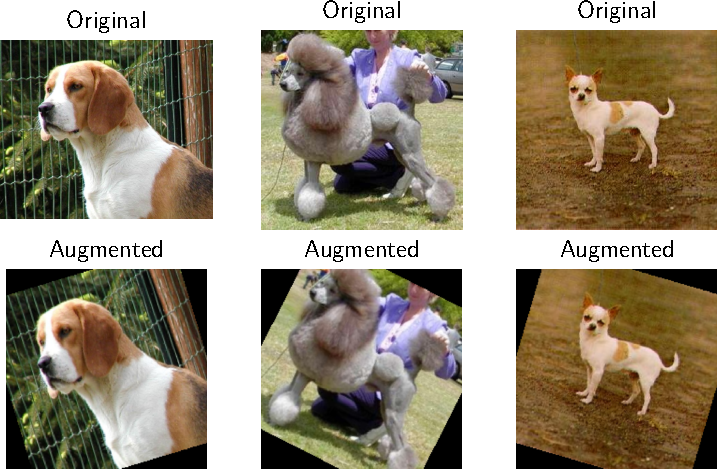
\includegraphics[width=\the\textwidth]{pics/subplot.pdf}
  \caption{Beispielbilder zur Data Augmentation. In der oberen Zeile sind die
  Originalbilder aus dem Datensatz und unten die Bilder nach dem Resizen und der Data Augmentation.}
  \label{fig:data_augmentation}
\end{figure}

Da der Datagenerator nach jeder Epoche neu aufgerufen wird, sehen die
Trainingsbilder in jeder Epoche anders aus, was allgemein die Robustheit des
\CNN gegenüber Translation, Rotation, etc. der Bilder erhöht und nebenbei mehr
Statistik generiert, da die Bilder immer anders aussehen.

\section{Netzwerkstrukturen}
Insgesamt wurden drei verschiedene Netzwerkarchitekturen verwendet, namentlich
\MiniDog, \PreDog und \PreBig. Die letzten beiden Architekturen verwenden dabei
ein vortrainiertes Netz mit Namen \texttt{InceptionResNetV2}. Dieses ist bei
Keras vorimplementiert \cite{inception} und wurde auf \texttt{ImageNet}
trainiert, einem Datensatz insgesamt bestehend aus 14197122 Bildern
\cite{imagenet}.

Da \texttt{InceptionResNetV2} alleine bereits 55873736 freie Parameter hat, muss
bei \PreBig und \PreDog Regularisierung verwendet werden. Die Struktur ist für
beide Neuronalen Netze die gleiche: An \texttt{InceptionResNetV2} ist eine Lage
\texttt{AveragePooling2D} mit einer \texttt{Poolsize=(4, 4)} und eine Lage
\texttt{GlobalMaxPooling2D} angeschlossen, um die Anzahl der freien Parametern
zu reduzieren. Danach kommen drei \texttt{Dense}-Layer, mit den
Dimensionalitäten 30, 30, 5 (für \PreDog) und 150, 120, 120 für \PreBig. Die
Layern sind \texttt{L2-Regularisiert} mit einem Wert von 0.01 für \PreDog und
0.007 für \PreBig. Außerdem befinden sich je ein \texttt{Dropout}-Layer mit
einer Stärke von 0.2 (\PreDog) bzw. 0.15 (\PreBig) zwischen den
\texttt{Dense}-Layern. Die Aktivierungsfunktion der \texttt{Dense}-Layer ist
\texttt{PReLU}, die Initialisierung wurde nach der von Kaiming He entwickelten
Methode durchgeführt \cite{tensowflow-he}, so wie in \cite{he-ini} empfohlen.
Auch die Gewichte des Kernels der \texttt{Dense}-Layer wurden nach der von
Kaiming He entwickelten Methode initialisiert. \texttt{PReLU} ist eine
modifizierte Version von \texttt{ReLU}, die sich dadurch auszeichnent, dass die
Funktion $f(y)$ für negative $y$ nicht 0 ist wie bei \texttt{ReLU}, sondern $ay$
mit einem Koeffizienten $a$, der adaptiv angepasst wird \cite{prelu}. Die
Aktivierungsfunktion des letzten \texttt{Dense}-Layers ist \texttt{softmax}.
